%%%%%%%%%%%%%%%%%%%%%%%%%%%
% Motivation and construction of the FRT Index
% Christopher Gandrud
% 31 March 2014
%%%%%%%%%%%%%%%%%%%%%%%%%%%%

\documentclass[a4paper]{article}
\usepackage{fullpage}
\usepackage[authoryear]{natbib}
\usepackage{setspace}
    \doublespacing
\usepackage{hyperref}
\hypersetup{
    colorlinks,
    citecolor=black,
    filecolor=black,
    linkcolor=cyan,
    urlcolor=cyan
}
\usepackage{amsmath}
\usepackage{dcolumn}
\usepackage{booktabs}
\usepackage{url}
\usepackage{tikz}
\usepackage{todonotes}
\usepackage[utf8]{inputenc} 
\usepackage{graphicx}
\usepackage{longtable}
\usepackage{todonotes}

%%%%%%%%% Title
\title{Measuring Financial Regulatory Transparency}

\author{Mark Copelovich \\ \emph{University of Wisconsin, Madison} \\[0.5cm] Christopher Gandrud and Mark Hallerberg \\ 
    {\emph{Hertie School of Governance}}\footnote{Friedrichstra{\ss}e 180. 10117 Berlin, Germany. Contact email: \href{mailto:gandrud@hertie-school.org}{gandrud@hertie-school.org}. All material for replicating the FRT Index and the analysis in this paper can be found at: \url{https://github.com/FGCH/FRTIndex}.}}


\begin{document}

\maketitle

%%%%%%%%% Abstract
\begin{abstract}
\noindent \emph{Early and incomplete working draft. Comments welcome.} \\
    Regulators need to have accurate information about financial institutions' activities for financial supervision to be effective. For the public to be able to hold supervisors accountable they need access to the information financial supervisors have about the health of their banking system. This makes it possible for them to judge the quality of regulators' actions. In this paper we use Bayesian Item Response Theory to create a new, global, and comparable Financial Regulatory Transparency (FRT) Index. The Index currently covers the years 1998 through 2011. It captures 60 high income countries'--those most likely to have developed financial systems--reporting to the World Bank's Global Financial Development Database. The Index is a distinct indicator of governments' willingness to gather and make publicly available credible information about their financial systems. In addition to describing the motivation behind and creation of the Index, we establish its value added as a unique and objective measure of financial supervisory transparency. We also begin to explore how financial regulatory transparency is related to supervisory quality and financial system stability.  
\end{abstract}

In previous research a number of us have found that even within the relatively homogeneous European Union where there are supranational authorities tasked with gathering and reporting aggregate financial data from member states that there is considerable variation in what is actually reported \cite[see][]{Gandrud2014a}. We currently lack a comparable cross-national way of measuring country's level of financial regulatory transparency. In this paper we use a Bayesian Item Response Theory (IRT) approach recently employed by \cite{Hollyer2014} to develop a new Financial Regulatory Transparency (FRT) Index. 

The Index includes 60 high income countries from 1998 through 2011. It measures these countries' reporting of financial system items to the World Bank's Global Financial Development Database (GFDD). The Index is a unique indicator of countries' willingness to credibly--the data has to pass minimal World Bank and International Monetary Fund quality checks--reveal the structure of their financial system and their regulatory quality, so that they can be scrutinized by market participants and citizens.

In this paper we first discuss why government transparency has been argued for and found to be important for good governance and also how previous researchers have attempted to measure it. We then discuss the construction of the FRT Index. In the following section we describe a selection of the Index's notable features and demonstrate its `value added' over less computationally intensive methods. Finally, we make preliminary explorations of associates between the Index and measures of financial regulatory quality and financial system stability. These investigations motivate future research.  

\section{Motivation: the importance of transparency}

\todo[inline]{Lit. review of (a) why transparency is important and (b) how it has been measured before.}

\section{Creating the FRT Index}

We treat financial regulatory transparency as an unobserved latent variable that effectively summarizes countries likelihood of reporting yearly data to indices included in the World Bank's Global Financial Development Database first created by \cite{Cihak2012}.\footnote{Access to the most updated version of the data set is available through \url{http://data.worldbank.org/data-catalog/global-financial-development}. Accessed February 2014.} In this section we describe how we selected the items and country-years to include in the Index as well as the estimation model that creates it.

\subsection{Included indicators}

To measure financial supervisory transparency we first gather data on whether or not governments reported data on a subset of indicators that are included in the World Bank's GFDD. We follow Hollyer et al.`s \citeyearpar{Hollyer2014} criteria for inclusion of items and country-years. First, we only include indicators that are reported by at least one country for each year in the period 1998-2011. This gave us the greatest coverage of indicators that are comparable across countries. Second, we exclude all indicators that were explicitly gathered for only a subset of countries. As such we avoid including data where the primary source is the Bank for International Settlements. Third, we do not include any indicator that is from a non-governmental source. This included both indicators from World Bank sponsored surveys, such as the Global Financial Inclusion Survey and the Enterprise Survey. This also includes data primarily derived from sources such as Swiss Re's Sigma Reports, Standard \& Poor's, Bankscope, and Bloomberg. Fourth, we do not include variables that are linear combinations of other variables. Fifth, we do not include variables that are simply references to the same quantity in different units. 

Additionally for the FRT Index, sixth, we aim to focus on countries that have relatively highly developed banking systems. As such we include only countries and jurisdictions that the World Bank classifies as `high income'.\footnote{We include both OECD and non-OECD high income countries.} Countries with lower levels of income likely do not have financial systems sophisticated enough to have a number of the quantities reported in the items. 

Using these criteria our model has 60 countries, 21 items, and 12 years (1998-2011). Table~\ref{IndTable} shows the list of indicator items and descriptions.  

\begin{table}[ht]
    \caption{Indicators included in the FRT Index from the World Bank's Global Financial Development Database}
    \label{IndTable}
    \vspace{0.3cm}
    \scalebox{0.95}{
        % latex table generated in R 3.0.2 by xtable 1.7-1 package
% Thu Feb 20 10:58:09 2014
{\scriptsize
\begin{tabular}{llll}
  \hline
SeriesCode & Indicator.Name & Source & Periodicity \\ 
  \hline
GFDD.DI.01 & Private credit by deposit money banks to GDP (\%) & IFS/IMF & 1961-2011 \\ 
  GFDD.DI.02 & Deposit money banks' assets to GDP (\%) & IFS/IMF & 1961-2011 \\ 
  GFDD.DI.03 & Nonbank financial institutions’ assets to GDP (\%) & IFS/IMF & 1961-2011 \\ 
  GFDD.DI.04 & Deposit money bank assets to deposit money bank assets and central bank assets (\%) & IFS/IMF & 1960-2011 \\ 
  GFDD.DI.05 & Liquid liabilities to GDP (\%) & IFS/IMF & 1961-2011 \\ 
  GFDD.DI.06 & Central bank assets to GDP (\%) & IFS/IMF & 1961-2011 \\ 
  GFDD.DI.07 & Mutual fund assets to GDP (\%) & World Bank & 1980-2011 \\ 
  GFDD.DI.08 & Financial system deposits to GDP (\%) & IFS/IMF & 1961-2011 \\ 
  GFDD.DI.11 & Insurance company assets to GDP (\%) & World Bank & 1980-2011 \\ 
  GFDD.DI.12 & Private credit by deposit money banks and other financial institutions to GDP (\%) & IFS/IMF & 1961-2011 \\ 
  GFDD.DI.13 & Pension fund assets to GDP (\%) & World Bank & 1990-2011 \\ 
  GFDD.DI.14 & Domestic credit to private sector (\% of GDP) & World Bank & Annual: \\ 
  GFDD.EI.02 & Bank lending-deposit spread & IFS/IMF & 1980-2011 \\ 
  GFDD.EI.08 & Credit to government and state owned enterprises to GDP (\%) & IFS/IMF & 1980-2011 \\ 
  GFDD.OI.02 & Bank deposits to GDP (\%) & IFS/IMF & 1961-2011 \\ 
  GFDD.OI.07 & Liquid liabilities in millions USD (2000 constant) & IFS/IMF & 1960-2011 \\ 
  GFDD.OI.13 & Remittance inflows to GDP (\%) & World Bank & 1970-2011 \\ 
  GFDD.SI.02 & Bank nonperforming loans to gross loans (\%) & IFSI/IMF & 1998-2011 \\ 
  GFDD.SI.03 & Bank capital to total assets (\%) & IFSI/IMF & 1998-2011 \\ 
  GFDD.SI.04 & Bank credit to bank deposits (\%) & IFS/IMF & 1960-2011 \\ 
  GFDD.SI.05 & Bank regulatory capital to risk-weighted assets (\%) & IFSI/IMF & 1998-2011 \\ 
  GFDD.SI.07 & Provisions to nonperforming loans (\%) & IFSI/IMF & 1998-2011 \\ 
   \hline
\end{tabular}
}

    }
    {\scriptsize{SeriesCode is the GFDD variable identifier.\\
    Sources Key:\\ 
    IFS = International Financial Statistics\\
    IMF = International Monetary Fund}}
\end{table}

\subsection{The model}

As in \cite{Hollyer2014} we let $y_{j,c,t} \in \{0,\; 1\}$ indicate a variable that is 1 when a country $c$ reports a GFDD variable $j$ in year $t$. It is 0 otherwise. We then estimate the model:

\begin{equation}
    \mathrm{Pr}(y_{j,c,t} = 1|transparency_{c,t}) = \mathrm{logit}(\delta_{j} + \beta_{j}transparency_{c,t})
\end{equation}

\noindent The following parameters are estimated in the model:

\begin{itemize}
    \item $\delta_{j}$ is the difficulty parameter of item $j$,
    \item $\beta_{j}$ the discrimination parameter for item $j$,
    \item $transparency_{c,t}$ is the estimated propensity of a given country-year $c,t$ to disclose financial regulatory data
\end{itemize}

\noindent $\delta_{j}$ indicates on average the degree to which countries report indicator $j$ in the GFDD over the entire time span. $\beta_{j}$ indicates how well reporting item $j$ predicts reporting other items. 

As \cite{Hollyer2014} note, simply taking the fraction of items a country reports in a given year as an indicator of transparency would be equivalent to assuming that $\delta_{j}$ and $\beta_{j}$ are constant across all variables. However, some items are `harder' to report than others as they reveal information that regulators may find difficult to gather without being more intrusive or, if they do gather it, they may consider it more sensitive for whatever reason. The IRT approach allows us to relax the equivalence assumption. Instead we directly estimate the degree to which countries find it `difficult' to report items and how reporting an item (or not) is related to non-reporting of other items.

In order to fix the scale and location of the the FRT Index we followed \cite{Hollyer2014} by subtracting it by the mean and dividing by the standard deviation of the first year of the data set (1998) at each iteration. 

The Index values in 1998 are draw from a diffuse normal prior ($Transparency_{c,1980} \sim N(0,\:100)$) before recentering. For each transparency value after 1998 we used a system of random-walk priors such that $transparency_{c,t} \sim N(transparency_{c,t-1},\: \frac{1}{\tau_{c}}) \forall t > 1$, where $\tau_{c}$ acts as a country-specific smoothing parameter. Each $\tau_{c}$ is estimated with the prior $\tau_{c} \sim Gamma(20,\:0.25)$ \citep[for more details see][8]{Jackman2009,Hollyer2014}. Finally, we used diffuse priors when estimating the discrimination and difficulty parameters:

\begin{equation}
    \begin{pmatrix}
      \delta{j} \\
      \beta_{j}
    \end{pmatrix} 
    \sim N 
    \left(
        \begin{pmatrix} 
            0 \\
            0 
        \end{pmatrix}
            ,\:
        \begin{pmatrix} 
            100 & 0 \\
            0 & 100
        \end{pmatrix}
    \right). 
\end{equation}

We estimated the model using a Markov Chain Monte Carlo algorithm using Just Another Gibbs Sampler (JAGS) 3.4.0 \citep{Plummer2003}.\footnote{The original JAGS model can be found at: \url{https://raw.githubusercontent.com/FGCH/FRTIndex/master/source/BasicModel_V1.bug}. The R \citep{RCite} source code needed to download the underlying indicators and run the JAGS model is available at: \url{https://raw.githubusercontent.com/FGCH/FRTIndex/master/source/FRTIndex_CreatorV2.R}. The later source code dynamically generates the JAGS model.} We estimated two chains using 10,000 iterations each including burn-ins of 5,000 iterations. Please see the Supplementary Materials for convergence diagnostics.\todo{Need to do once the full model has been run.} 

\todo[inline]{Model fit discussion here}

\section{Description and Validity}


\subsection{The FRT Index}

Figures \ref{FRT_1998}, \ref{FRT_2007}, and \ref{FRT_2011} provide snapshots of the Financial Regulatory Transparency Index in the years 1998 (the Index's first year), 2007, and 2011 (the Index's current end year). Higher scores on the FRT Index indicate higher financial regulatory transparency.

We should first notice that the index passes a face validity test. There is a noticeable cluster of countries with very low FRT scores. These countries include the Bermuda, Cayman Islands, the Isle of Man, and Monaco. All of these jurisdictions are known for their banking secrecy, often as explicit policy decisions to attract capital from those seeking to avoid paying taxes in their home jurisdictions. At the high end of the scale we also see countries that have been known for their transparency. \cite{Gandrud2014a} noted a high level of financial regulatory transparency in the United States' financial regulatory reporting practices relative to practices among many European Union countries. As we would expect from this work, the United States is regularly placed among the countries with the highest FRT scores.  

Changes in countries' FRT scores over time also reflect substantively meaningful policy changes. Hungary is a prime example. Figure~\ref{FRTHungary} shows Hungary's FRT Index across all of the years in the sample. In 1998 it is estimated to have one of the highest FRT scores, with a median well above 5. However, this declines over time with a clear break to very low transparency levels starting in 2009. The 2009 figures would have been reported to international institutions in 2010, the year that Viktor Orb\'{a}n's Christian Democratic People's Party entered government. This government introduced a number of major economic and financial policy changes that sometimes directly contradicted Hungary's international commitments, including reducing the independence of the central bank. \todo{Mark H. could you add some thoughts on this?}

\begin{figure}
    \caption{Financial Regulatory Transparency Index in 1998}
    \label{FRT_1998}
    \begin{center}
        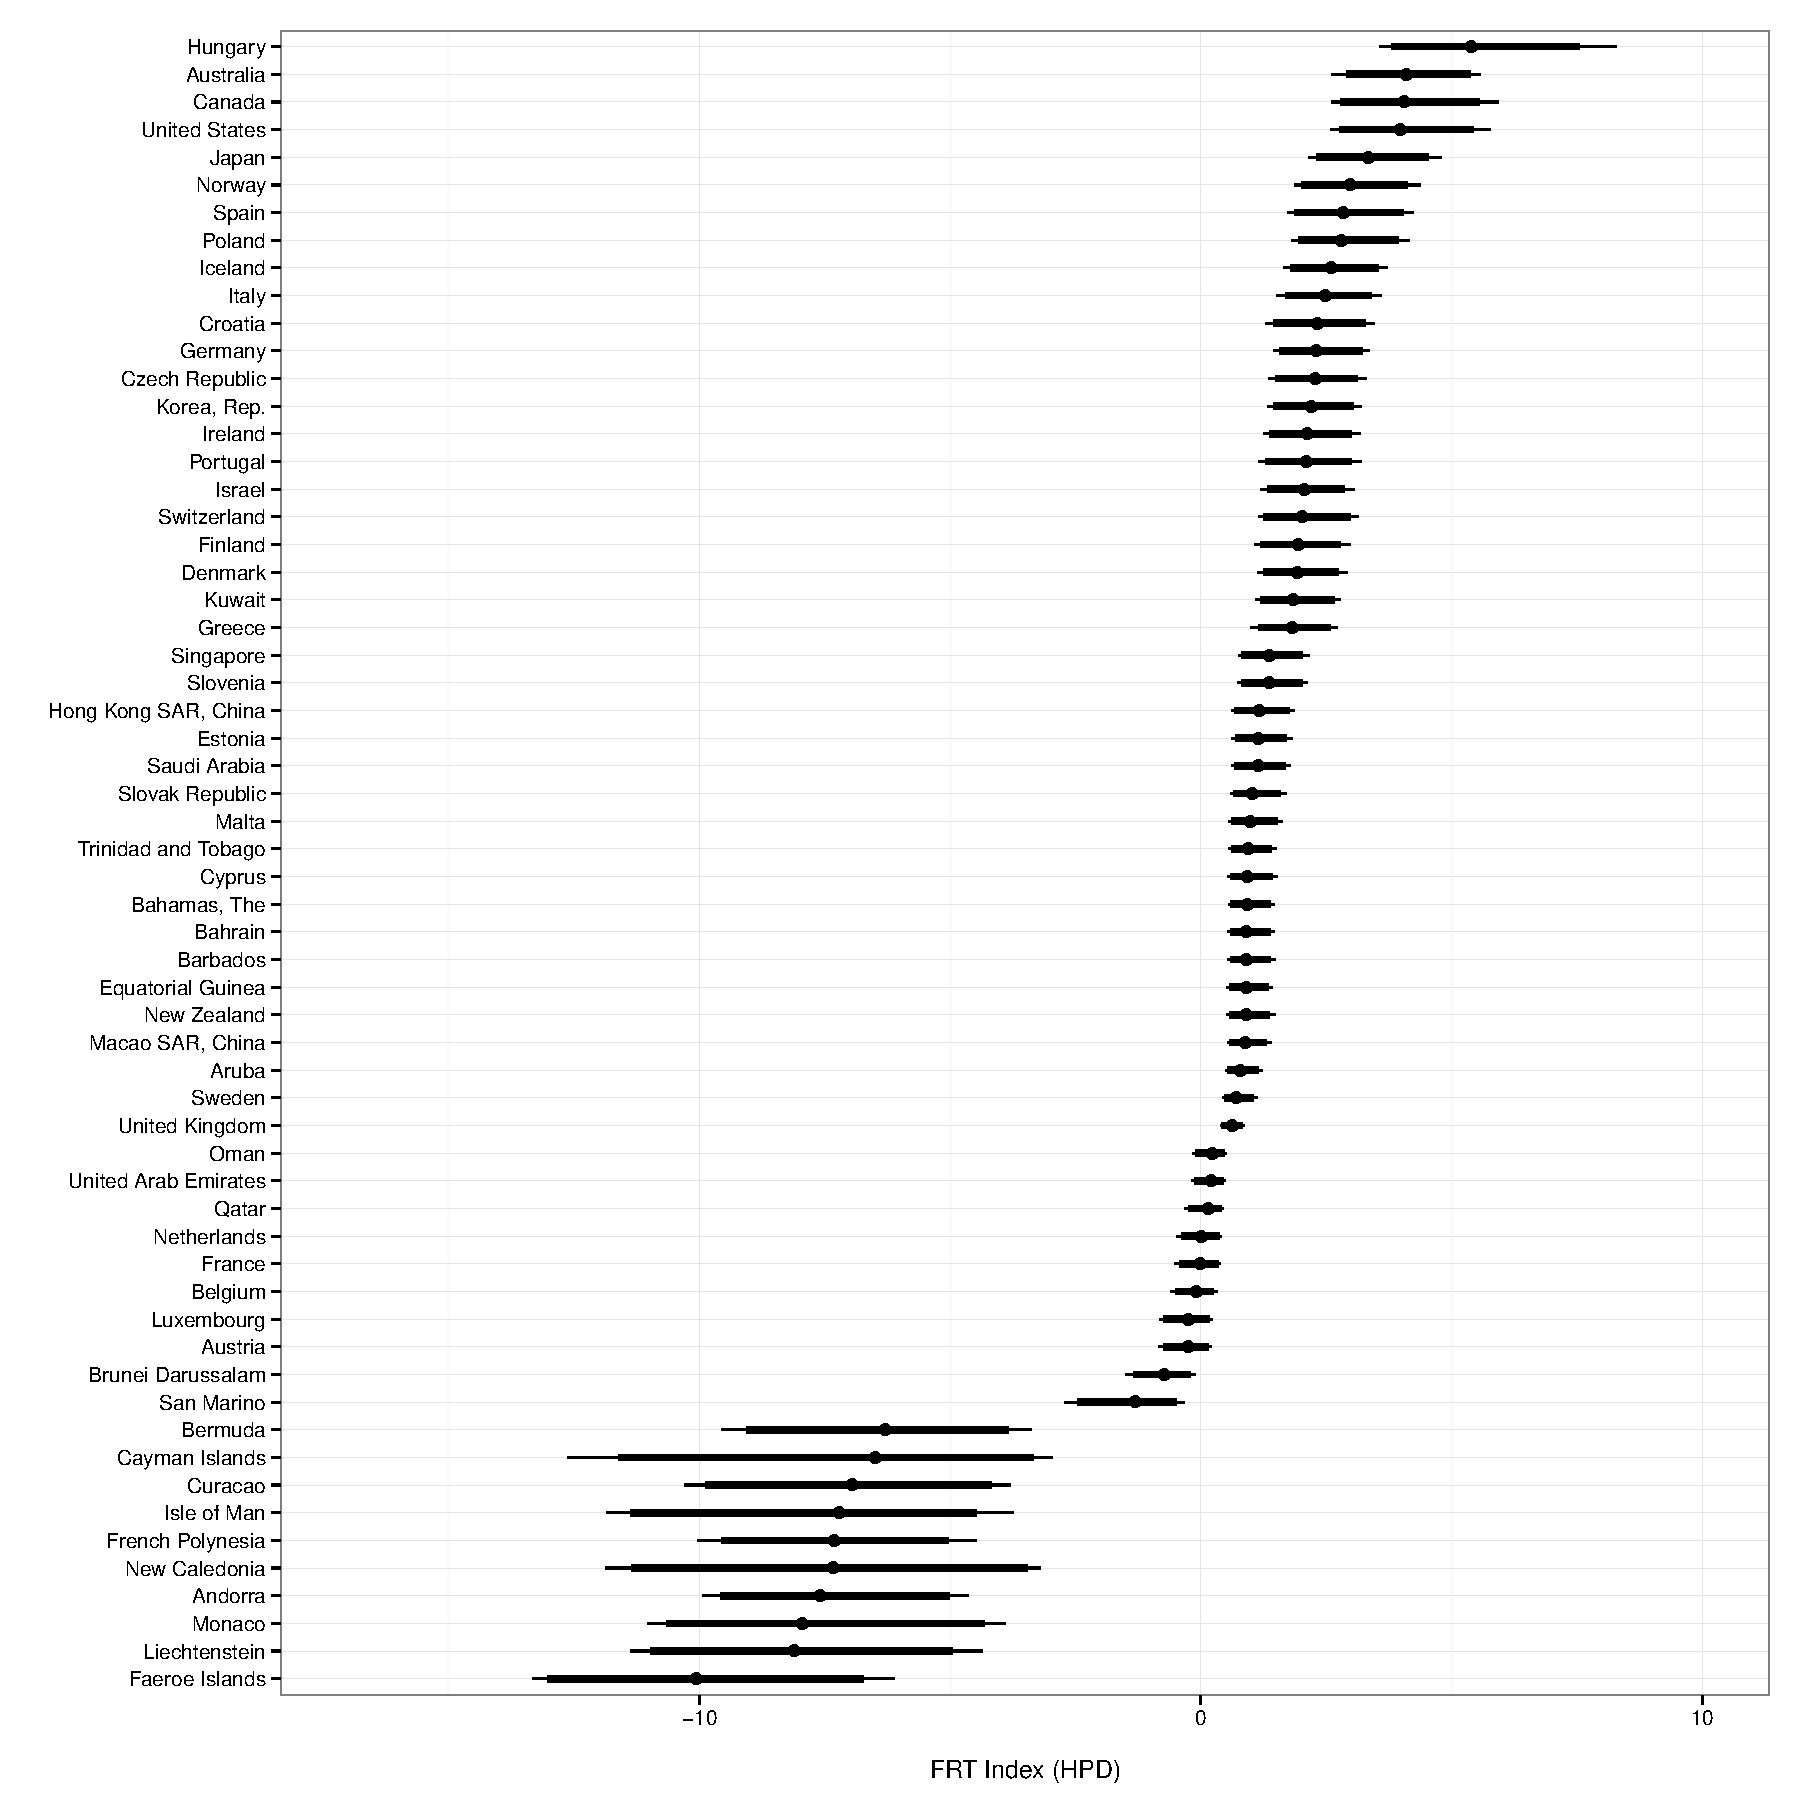
\includegraphics[scale=0.45]{figures/FRT_1998}
    \end{center}
    {\scriptsize{Thin lines represent the 95\% highest posterior density interval. Thick lines represent the 90\%. Points represent the median.}}
\end{figure}

\begin{figure}
    \caption{Financial Regulatory Transparency Index in 2007}
    \label{FRT_2007}
    \begin{center}
        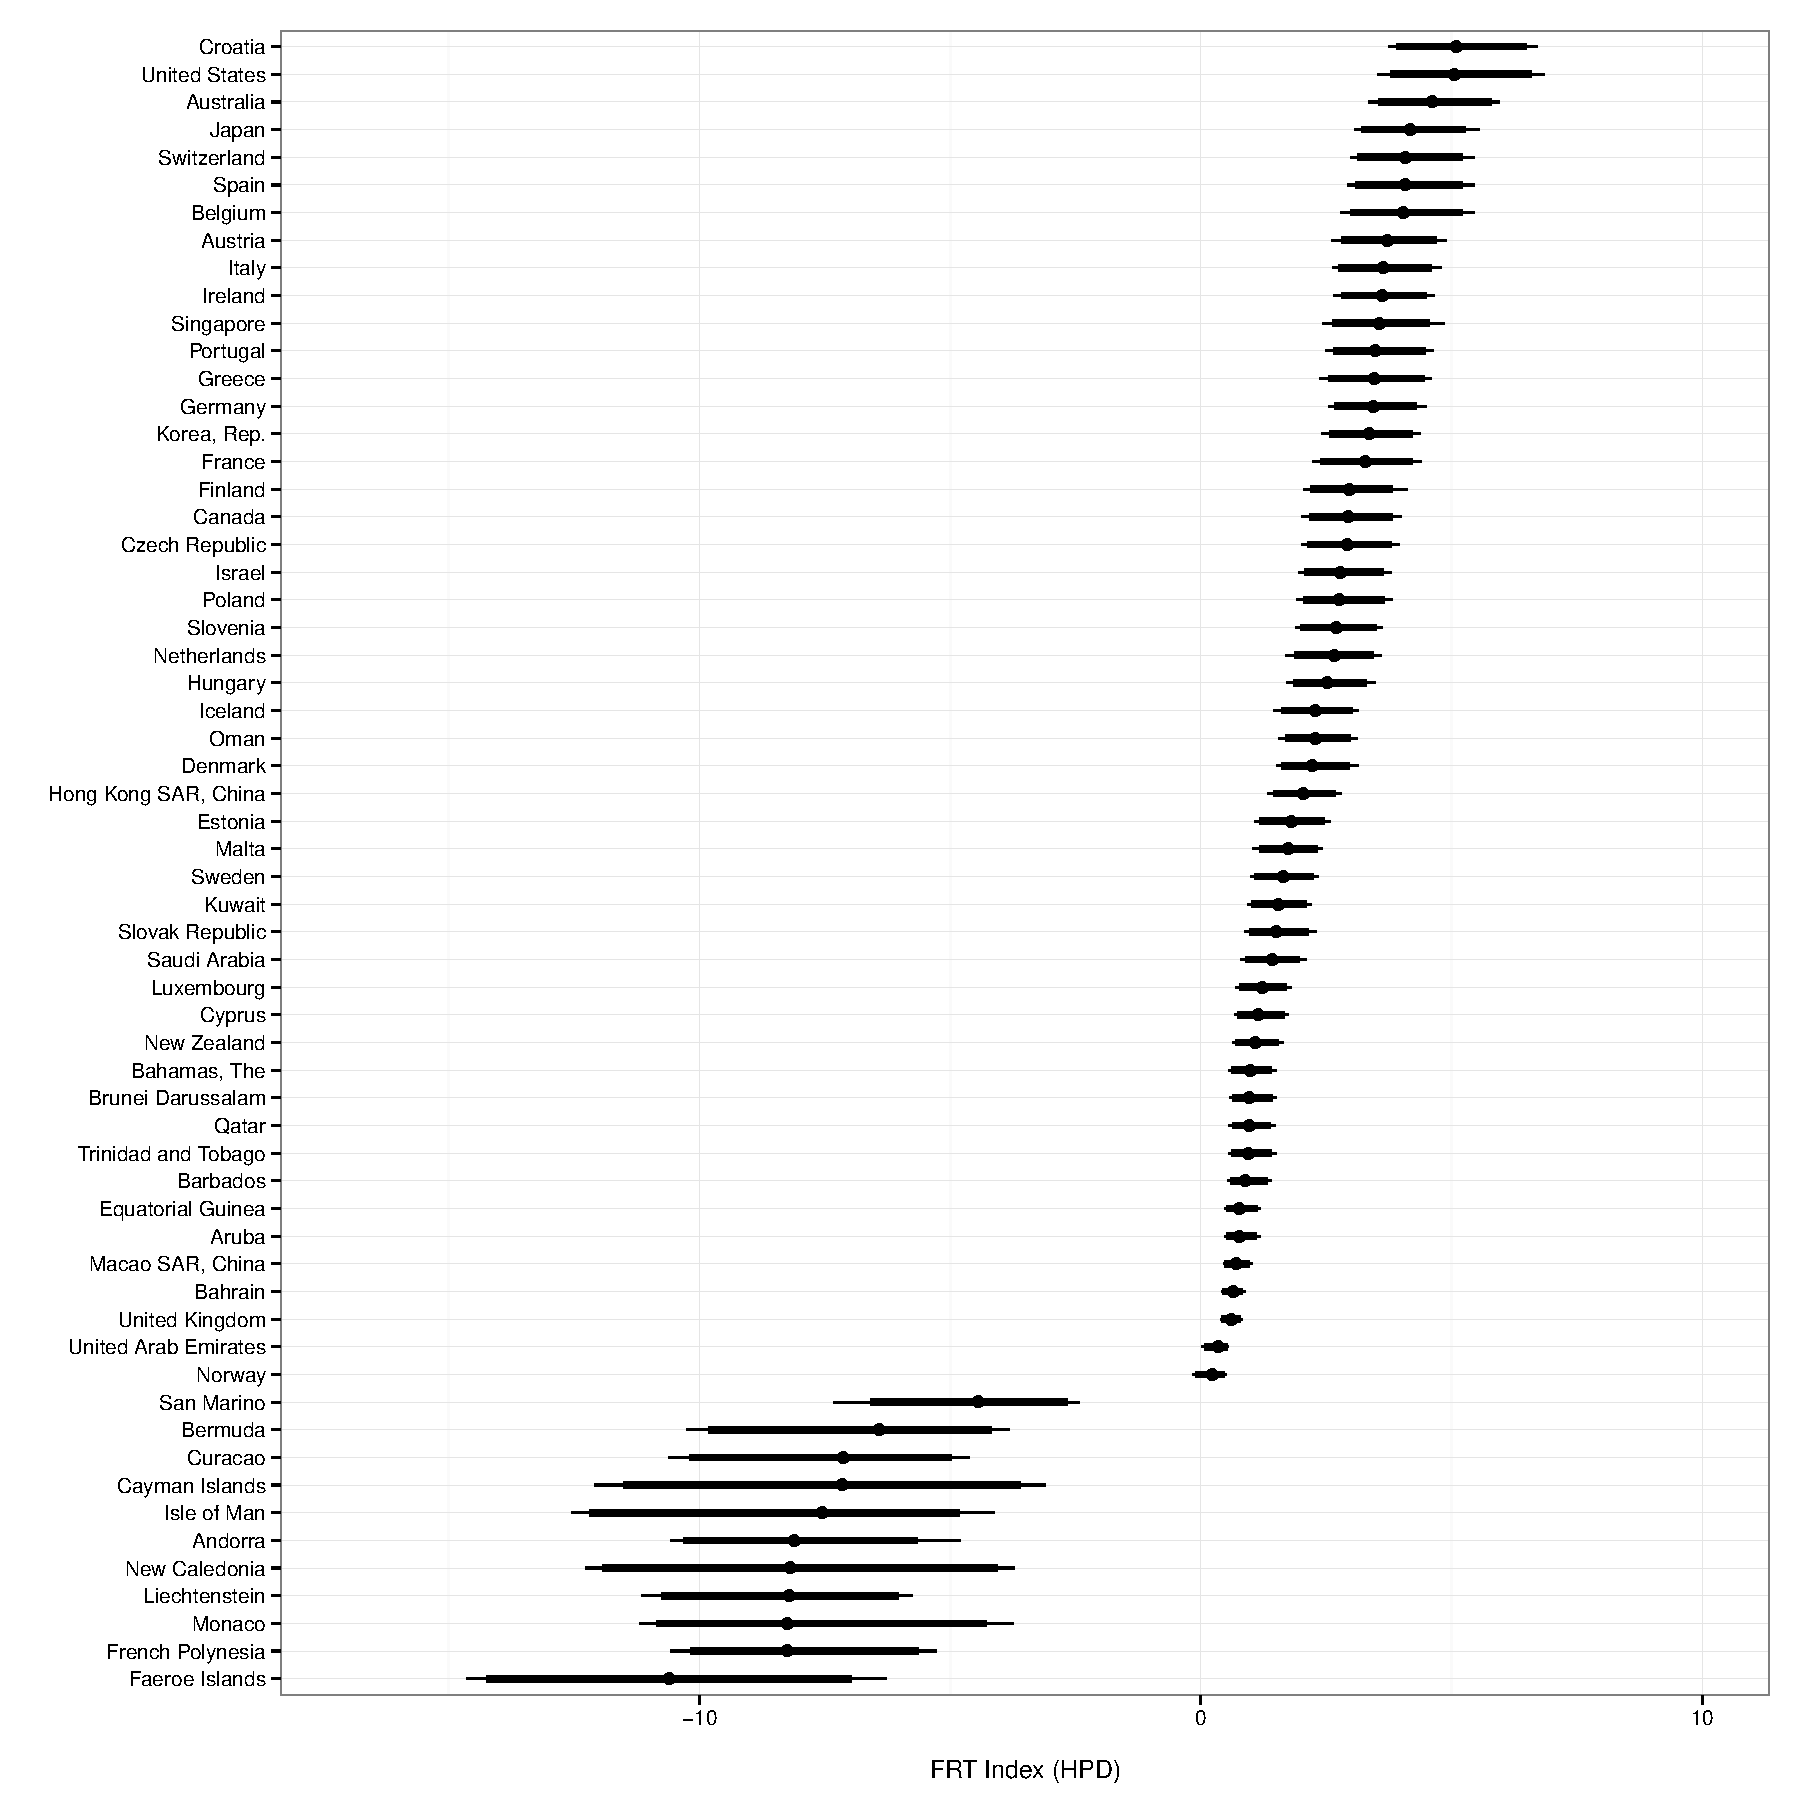
\includegraphics[scale=0.45]{figures/FRT_2007}
    \end{center}
    {\scriptsize{Thin lines represent the 95\% highest posterior density interval. Thick lines represent the 90\%. Points represent the median.}}
\end{figure}

\begin{figure}
    \caption{Financial Regulatory Transparency Index in 2011}
    \label{FRT_2011}
    \begin{center}
        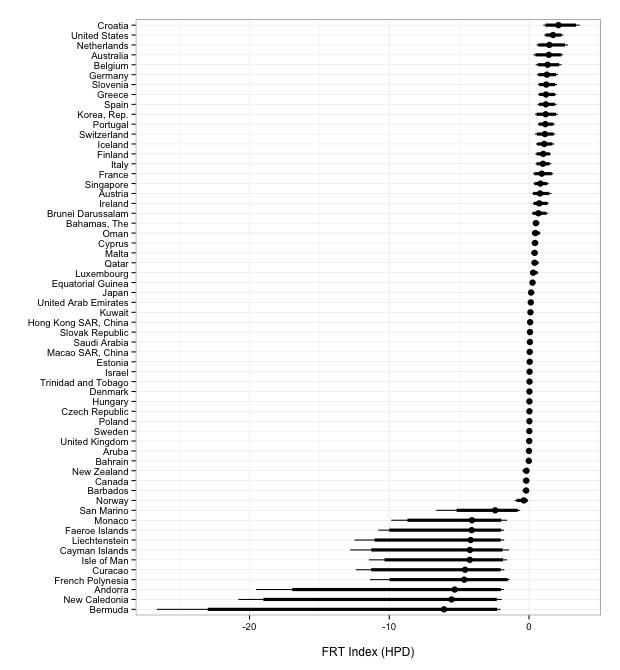
\includegraphics[scale=0.45]{figures/FRT_2011}
    \end{center}
    {\scriptsize{Thin lines represent the 95\% highest posterior density interval. Thick lines represent the 90\%. Points represent the median.}}
\end{figure}

It's important to also note that the FRT Index provides distinct information from more general transparency indices, such as Hollyer et al.'s HRV Index and Freedom House. \todo{Complete}  

\todo{COMPARE COUNTRY PLACEMENT TO HRV INDEX, ESPECIALLY SWEDEN.}

\begin{figure}
    \caption{Financial Regulatory Transparency Index for Hungary}
    \label{FRTHungary}
    \begin{center}
        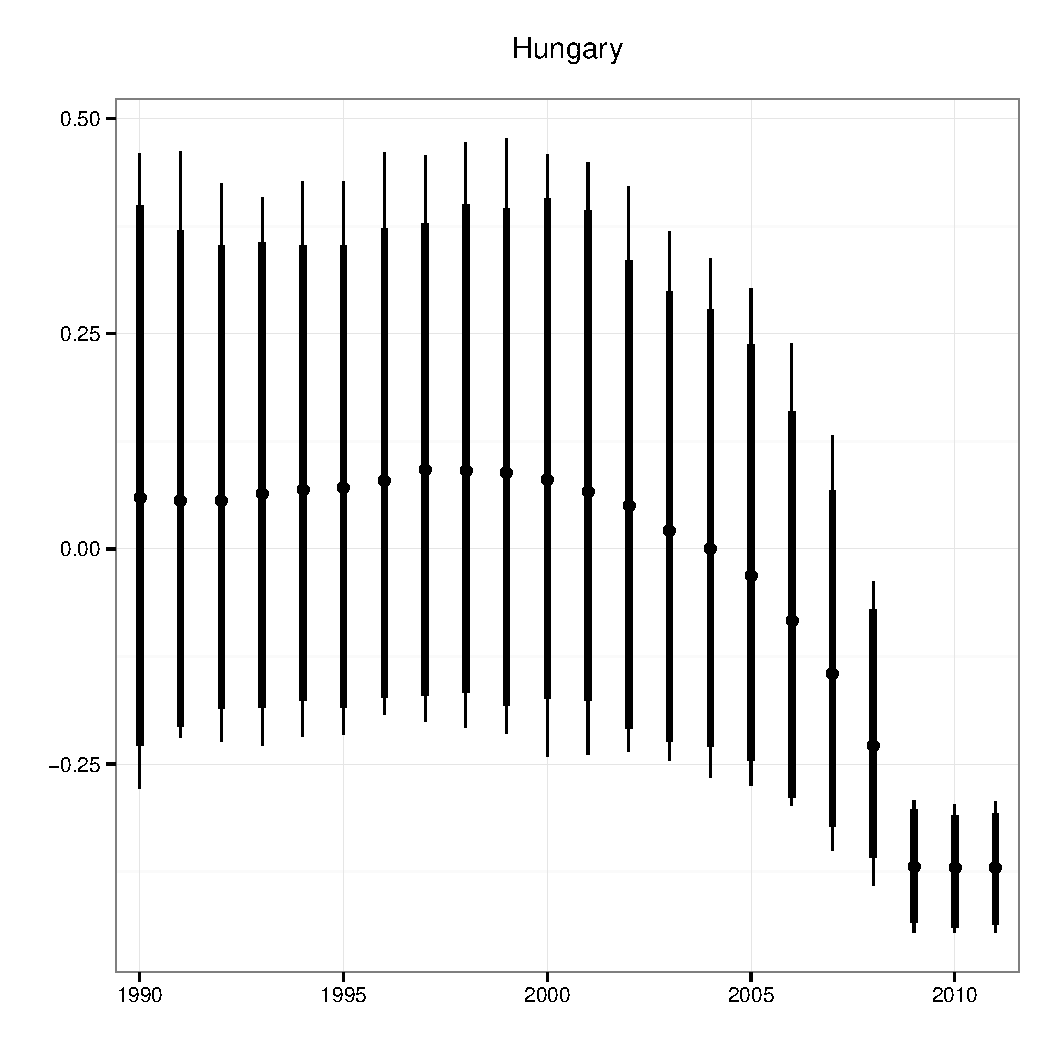
\includegraphics[scale=0.5]{figures/FRT_Hungary}
    \end{center}
    {\scriptsize{Thin lines represent the 95\% highest posterior density interval. Thick lines represent the 90\%. Points represent the median.}}
\end{figure}

\subsection{Value added: comparison to frequency methods}

A less computationally intensive method for developing a financial regulatory transparency index include would be to examine item reporting frequencies with sum-scores (summing the number of items reported per country-year) or some normalizing transformation of this like finding the proportion of items a country reported in a year. These approaches implicitly assume that reporting any one item is equivalent to reporting any other item. This may not be the case. Reporting one item may be `more difficult' than reporting another. Using IRT allows us to adjust for the fact that some items may be more readily reported than others. 

A basic test for examining if a frequency method would be just as appropriate and, because it is dramatically less computationally intensive, preferable to Bayesian IRT for constructing a transparency measure is to see if there is a linear association between the Bayesian IRT scores and frequency scores. Figure~\ref{CompFreqFRT} compares the proportion of items used (a frequency measure) in the FRT Index a country reported in a given year to that country-year's FRT score.\footnote{Both are standardized by subtracting their mean and dividing by their standard deviation.} Rather than having a linear relationship, we can see that the FRT Index is much more sensitive to indicator reporting than the frequency measure. This is especially true of countries that report relatively few items. They do substantially worse in the FRT Index than if we measured transparency with proportion of items reported.

\begin{figure}
    \caption{Comparing Frequency Reported vs. FRT Index}
    \label{CompFreqFRT}
    \begin{center}
        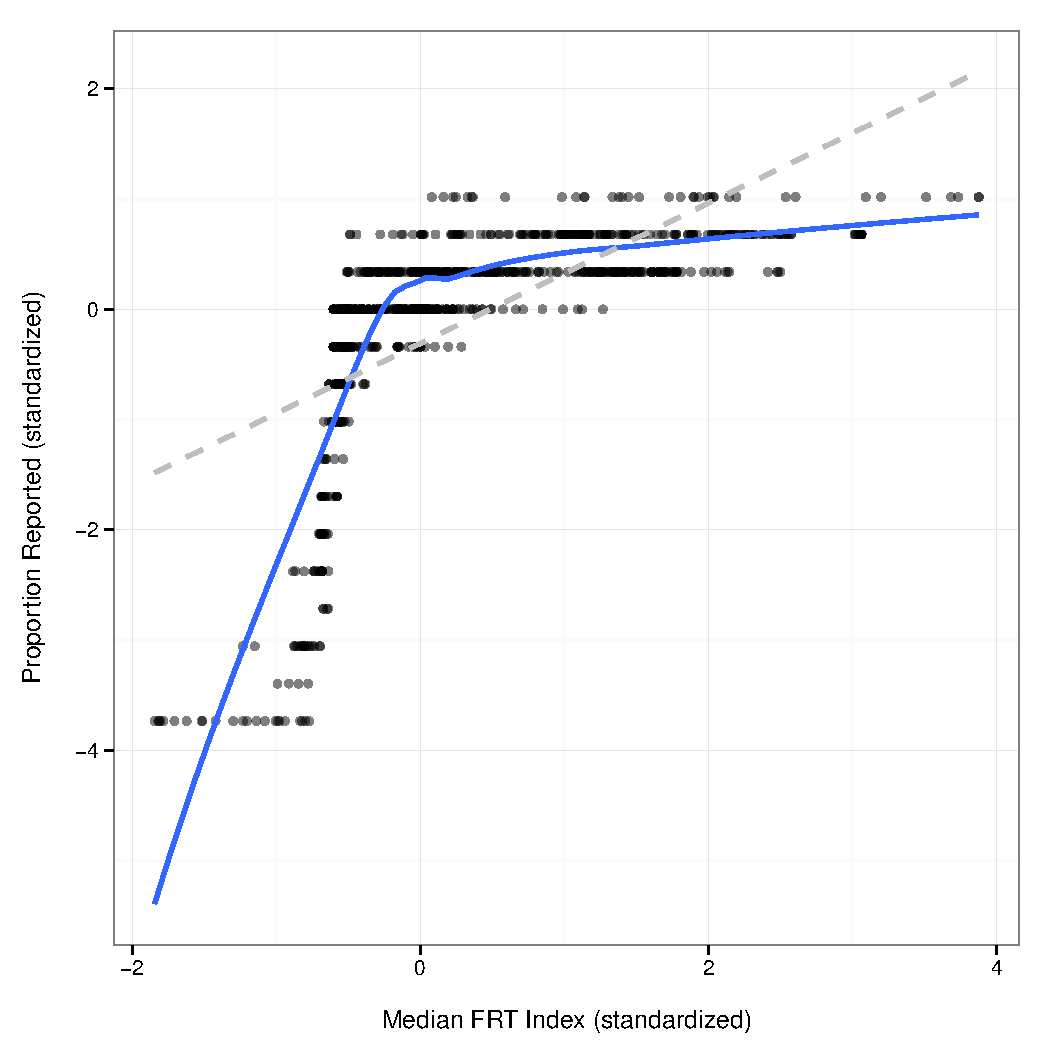
\includegraphics[scale=0.4]{figures/FRT_Prop_Compare} 
    \end{center}
    {\scriptsize{Both the Proportion Reported transparency indicator and the FRT Index scores were standardized by subtracting their means and dividing by their standard deviations.}}
\end{figure}


\subsection{Indicator difficulty and discrimination}

In addition to comparing the FRT Index to proportions of items reported, we can also examine the difficulty and discrimination parameters to determine whether or not the FRT has value added. If reporting one item is actually equivalent to reporting any other item then we would expect the estimated difficulty and discrimination parameters to be the same across all items. Figures \ref{DifficultyFig} and \ref{DiscrimFig} show the estimated difficulty and discrimination parameter estimates for all of the included items, respectively. 


\begin{figure}
    \caption{Estimated Item Difficulty Parameters}
    \label{DifficultyFig}
    \begin{center}
        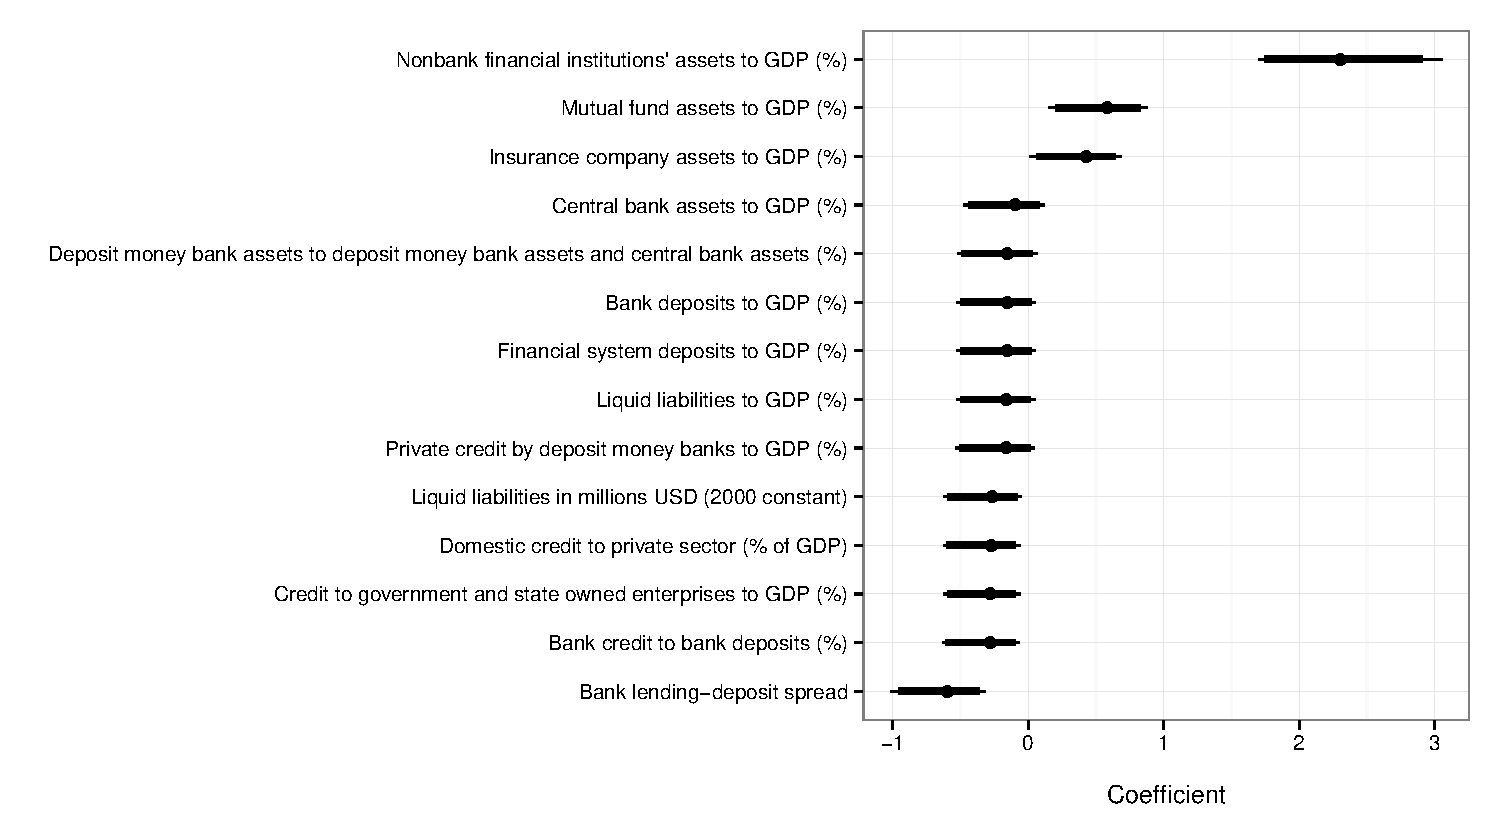
\includegraphics[scale=0.5]{figures/difficultyPlot}
    \end{center}
\end{figure}



\begin{figure}
    \caption{Estimated Item Discrimination Parameters}
    \label{DiscrimFig}
    \begin{center}
        \includegraphics[scale=0.5]{figures/discriminationPlot}
    \end{center}
\end{figure}


\section{Preliminary Associations}

To demonstrate the potential usefulness of the FRT Index we examine a number of associations between the Index and the occurrence and potential occurrence of financial crisis.

\todo[inline]{[ASSOCIATION WITH ECONOMIC BUREAUCRATIC CAPACITY]
[Z-SCORE (PROB. OF BANK DEFAULT) AS DEPENDENT VARIABLE]}

A standard measure of a banking system's health is the jurisdiction level `Z-Score'. This measure attempts to capture the probability of individual bank insolvency, but is sometimes aggregated to the jurisdiction level. The World Bank's GFDD includes a Z-score calculated by using Bankscope, Bureau van Dijk unconsolidated bank-level data. Aggregated to the jurisdiction level it compares commercial banks' buffers (capitalization and returns) to the volatility of those returns. A higher Z-score indicates that there is a higher probability of insolvency.

\begin{figure}
    \caption{Initial Associations}
    \label{basicAssoc}
    \begin{center}
        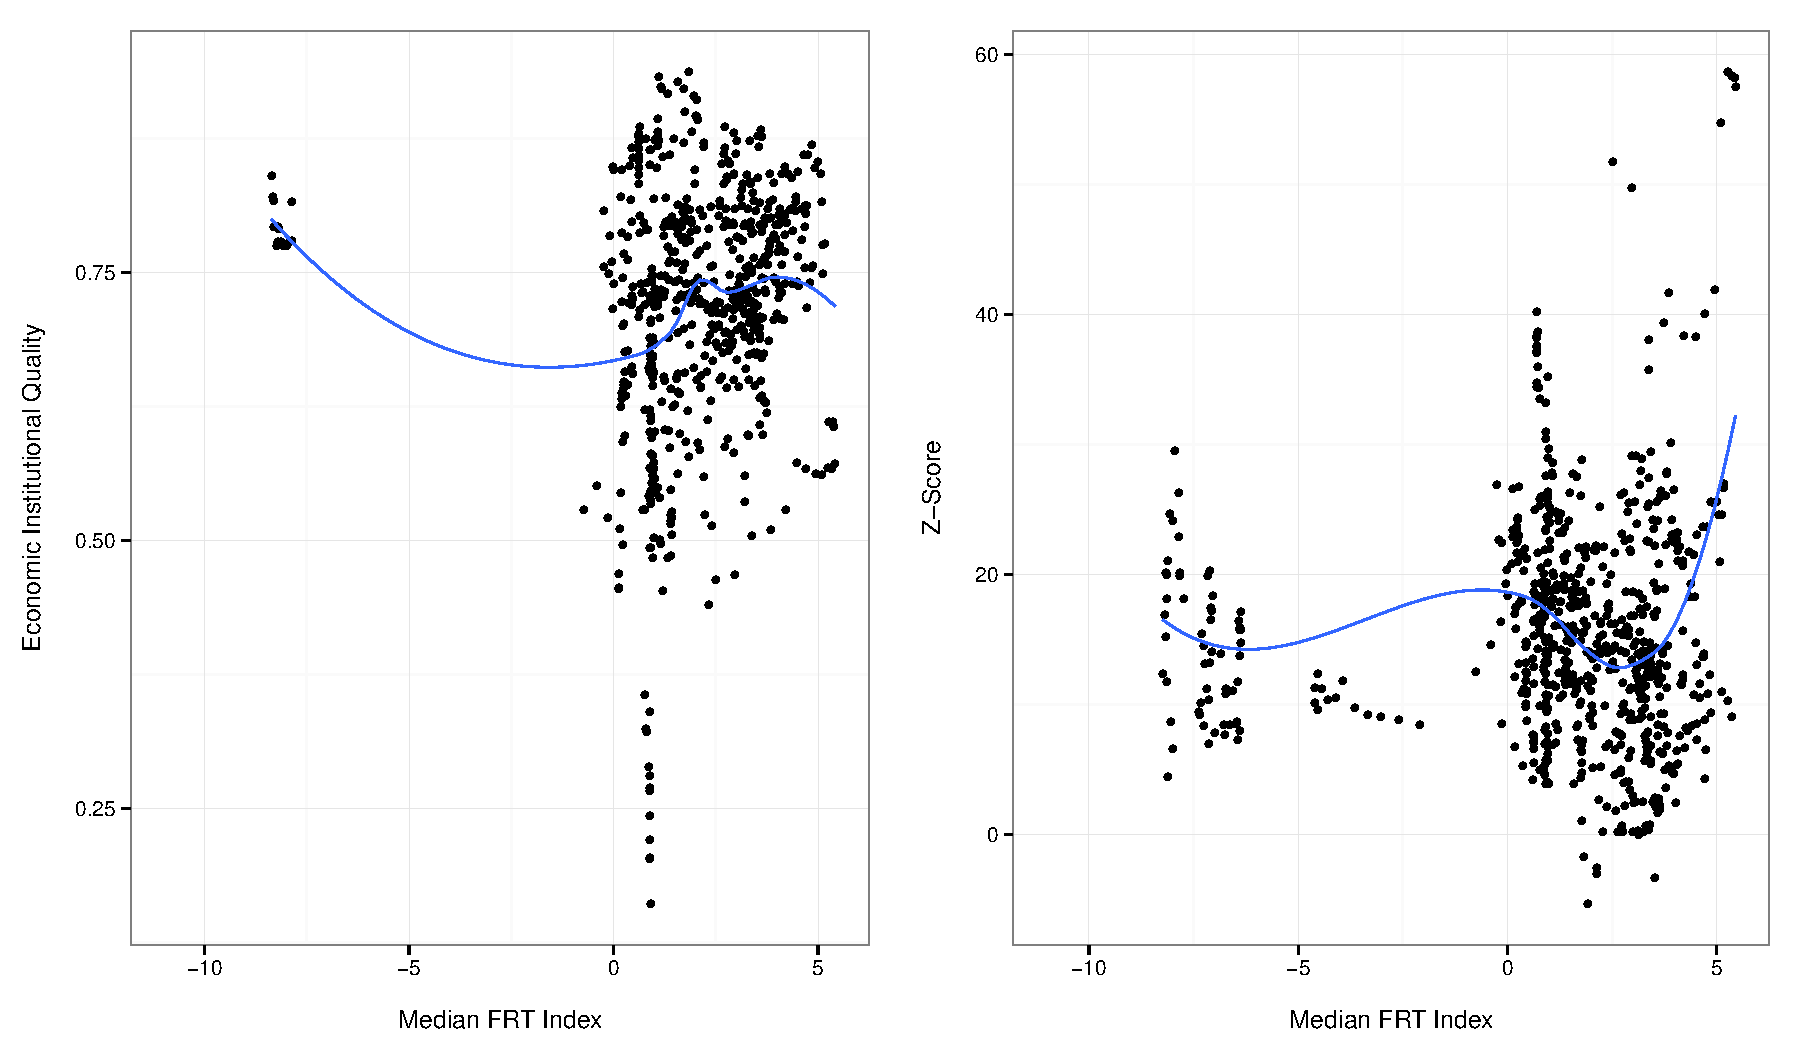
\includegraphics[scale=0.5]{figures/Associations1}
    \end{center}
\end{figure}

\section*{Conclusion}

In this paper we have introduced a new Financial Regulatory Transparency Index.

\todo[inline]{Complete}

\bibliographystyle{apsr}
\bibliography{FRTIndex}

\section*{Supplementary Materials}

\todo[inline]{TRACE PLOTS AND OTHER DIAGNOSTICS}


\end{document}
